%\subsection{Independent Sets} \label{IndSets}

\begin{definition}
    Let $G$ be a graph. A subset $S$ of $G$ is called \textit{independent} if no two distinct vertices of $G$ are adjacent. The maximum independent set problem is the problem of finding an independent set of greatest size in a graph $G$.
\end{definition}

\begin{example}
    Take $G$ to be the following graph. Both the red and blue sets are independent in $G$, but only the blue set is maximum.
    
    \begin{center}
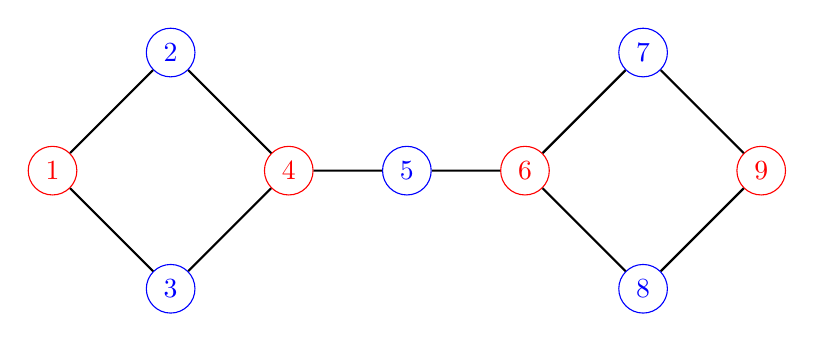
\begin{tikzpicture}[scale=1.5]

    \node[circle, draw, red] (a) at (0,1) {1};
    \node[circle, draw, blue] (b) at (1,2) {2};
    \node[circle, draw, blue] (c) at (1, 0) {3};
    \node[circle, draw, red] (d) at (2,1) {4};
    \node[circle, draw, blue] (e) at (3,1) {5};
    \node[circle, draw, red] (f) at (4,1) {6};
    \node[circle, draw, blue] (g) at (5,2) {7};
    \node[circle, draw, blue] (h) at (5,0) {8};
    \node[circle, draw, red] (k) at (6,1) {9};

    \draw[thick] (a) -- (b);
    \draw[thick] (a) -- (c);
    \draw[thick] (b) -- (d);
    \draw[thick] (c) -- (d);
    \draw[thick] (d) -- (e);
    \draw[thick] (e) -- (f);
    \draw[thick] (f) -- (g);
    \draw[thick] (f) -- (h);
    \draw[thick] (g) -- (k);
    \draw[thick] (h) -- (k);

\end{tikzpicture}
\end{center}
\end{example}

The definitions of matching and independent set are visibly similar: they differ by replacing 'vertex' with 'edge' and 'shares a vertex' with 'adjacent'. This inspires a concrete way to relate the two problems.

\begin{construction}\label{edgegraph}
    Let $H$ be a hypergraph. We define its \textit{edge graph} $E(H)$ as follows:

    The vertices of $E(H)$ are the hyperedges of $H$.

    Two distinct hyperedges $e$ and $e'$ have an edge between them if and only if $e$ and $e'$ share a vertex.
\end{construction}

Expanding the definitions, an independent set in $E(H)$ is exactly a matching for $H$.

\begin{proposition}
    The maximum matching problem for hypergraphs and the maximum independent set problem are reducible to one another. 
\end{proposition}

\begin{proof}
    By construction, an independent set in $E(H)$ is exactly matching for $H$. Thus a maximum independent set in $E(H)$ is the same as a maximum matching for $H$, showing the maximum matching problem reduces to the maximum independent set problem.
    
    For the other direction, it suffices to show every graph can be realized as $E(H)$ for some $H$. Let $G$ be a graph and enumerate its edges $e_{1}, e_{2}, \ldots, e_{m}$. Take $H$ to be a $m$-partite hypergraph with edges corresponding to the vertices of $G$ so that for each $1 \leq i \leq m$, only the two edges of $e_{i}$ share a vertex. By construction the vertices of $E(H)$ correspond to those of $G$ with an edge between them if and only if the corresponding vertices have an edge in $G$.
\end{proof}

\begin{remark}
    In fact, the maximum independent set problem is reducible to 3-dimensional max matching, since both are NP-complete. \cite{karp21}
\end{remark}
